\chapter{État de l'art des attaques sur SSL/TLS}

\begin{figure}[H]
  \caption{Historique des attaques SSL/TLS (source : Cloudflare \cite{cloudflare})}
  \fbox{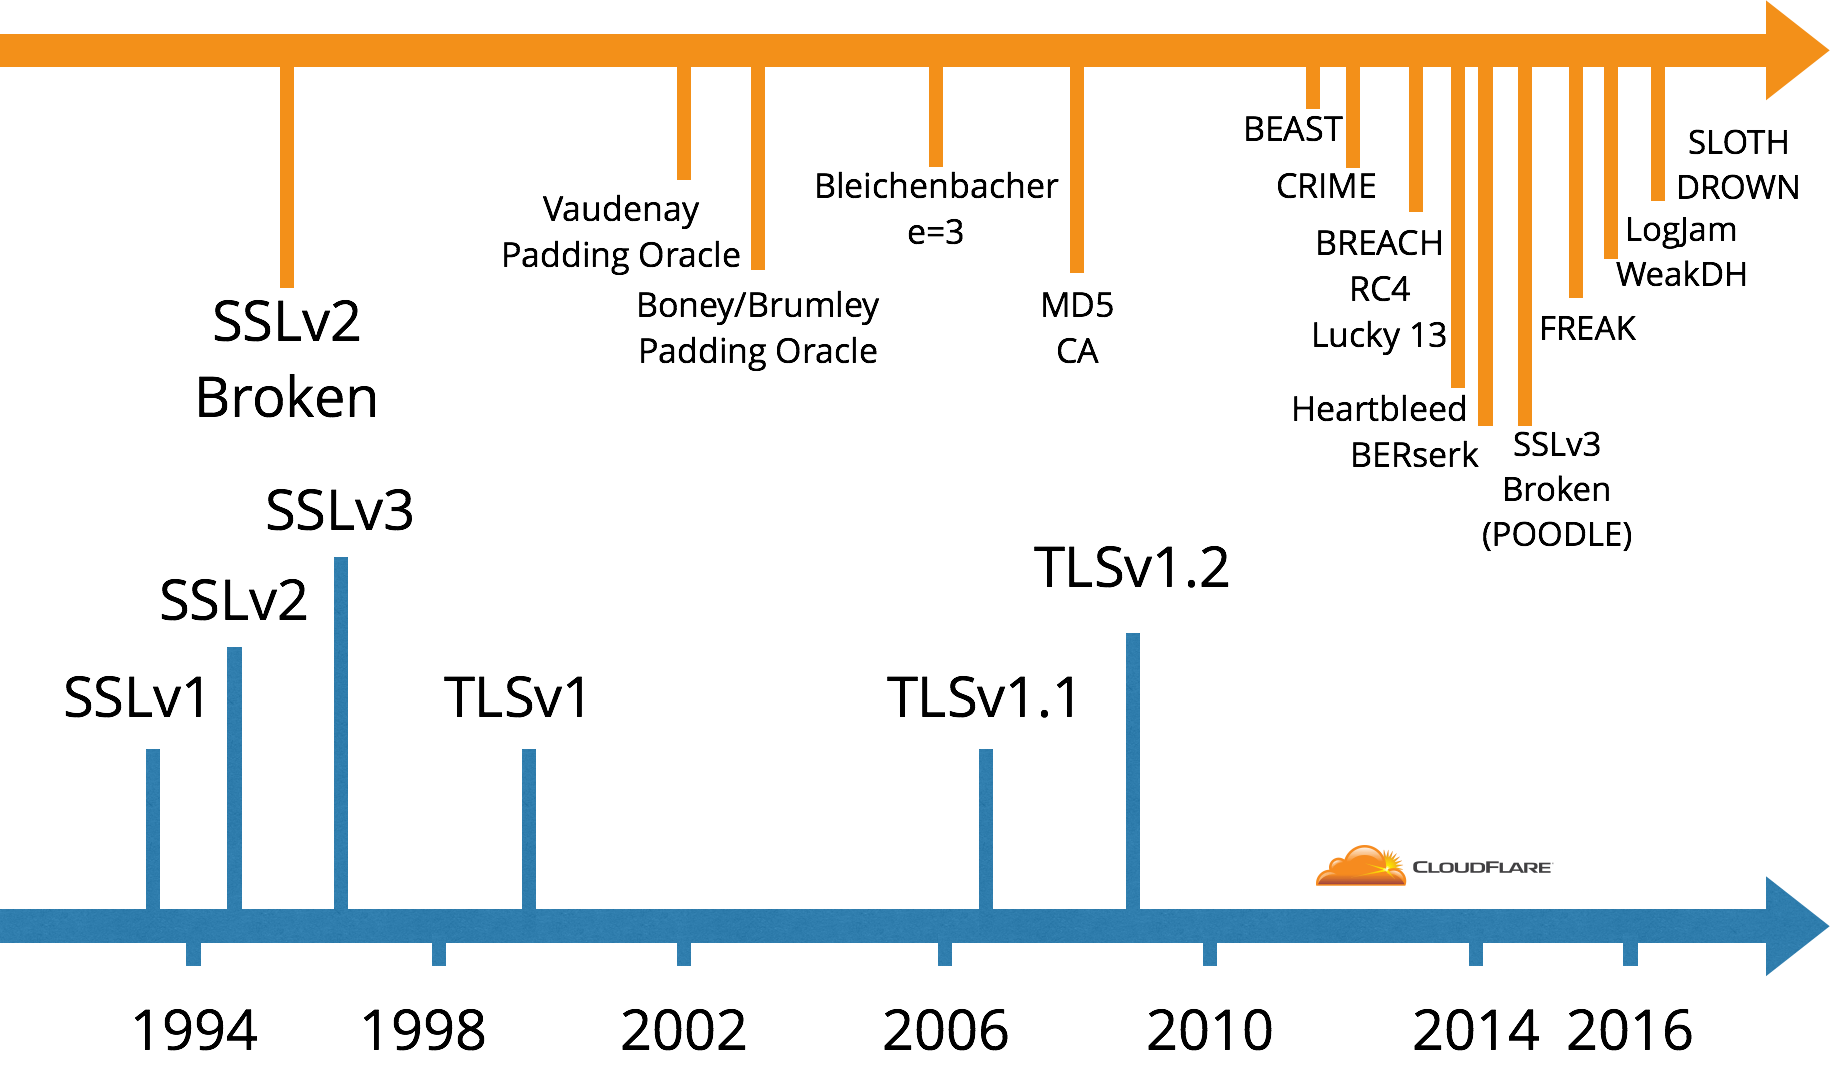
\includegraphics[width=\textwidth]{./history-tls-attacks.png}}
\end{figure}

\section{Attaques liées à l'implémentation}

\subsection{Heartbleed (2014)}
Cette faille est une faille d'OpenSSL basée sur SSL/TLS. Cette vulnérabilité permet de lire la mémoire du serveur. Cette faille est due à une erreur de programmation dans la focntion Heartbeat qui permet de maintenir la connexion sécurisée entre le navigateur et le serveur.

En effet, l'attaquant peut mentir sur le poids de la requête qu'il envoit et obtenir des données qui ne lui était pas destinées mais qui se trouve en mémoire. Il peut donc récupérer les informations comme des identifiants, des mots de passes, des cookies de sessions ou encore des clés de chiffrements \cite{heartbleed}.

\subsection{BERserk (2014)}

Blablabla \cite{berserk}

\section{Attaques liées à la cryptographie}

\subsection{BEAST (2011)}

Blablabla \cite{beast}

\subsection{Cassage de RC4 (2013)}

Blablabla \cite{rc4}

\subsection{Lucky13 (2013)}

Blablabla \cite{lucky13}

\subsection{Logjam (2015)}

Blablabla \cite{logjam}

\subsection{DROWN (2016)}

Blablabla \cite{drown}

\subsection{SLOTH (2016)}

Blablabla \cite{sloth}

\subsection{SWEET32 (2016)}

Blablabla \cite{sweet32}

\subsection{ROBOT (2017)}

Blablabla \cite{robot}

\section{Attaques sur le protocole}

\subsection{CRIME (2012)}

Blablabla \cite{crime}

\subsection{BREACH (2012)}

Blablabla \cite{breach}

\subsection{POODLE (2014)}

Blablabla \cite{poodle}

\subsection{FREAK (2015)}

Blablabla \cite{freak}

\subsection{WeakDH (2015)}

Blablabla \cite{weakdh}

\section{Attaques de l'homme du milieu}

\subsection{SSLsniff (2002)}

Blablabla \cite{sslsniff-website}

\subsection{SSLstrip (2009)}

Blablabla \cite{sslstrip-website}

\subsection{HTTPS interception}

Blablabla \cite{https-interception}
